\documentclass[a4paper, 12pt]{article}		% general format

%%%% Charset
\usepackage{cmap}							% make PDF files searchable and copyable
\usepackage[utf8x]{inputenc}				% accept different input encodings
\usepackage[T2A]{fontenc}					% russian font
\usepackage[russian]{babel}					% multilingual support (T2A)

%%%% Graphics
\usepackage[dvipsnames]{xcolor}			% driver-independent color extensions
\usepackage{graphicx}						% enhanced support for graphics
\usepackage{wrapfig}						% produces figures which text can flow around

%%%% Math
\usepackage{amsmath}						% American Mathematical Society (AMS) math facilities
\usepackage{amsfonts}						% fonts from the AMS
\usepackage{amssymb}						% additional math symbols

%%%% Typograpy (don't forget about cm-super)
\usepackage{microtype}						% subliminal refinements towards typographical perfection
\linespread{1.3}							% line spacing
\usepackage[left=2.5cm, right=1.5cm, top=2.5cm, bottom=2.5cm]{geometry}
\setlength{\parindent}{0pt}					% we don't want any paragraph indentation
\usepackage{parskip}						% some distance between paragraphs

%%%% Tables
\usepackage{tabularx}						% tables with variable width columns
\usepackage{multirow}						% for tabularx
\usepackage{hhline}							% for tabularx

%%%% Graph
\usepackage{tikz}							% package for creating graphics programmatically
\usetikzlibrary{arrows}						% edges for tikz

%%%% Other
\usepackage{url}							% verbatim with URL-sensitive line breaks
\usepackage{fancyvrb}						% sophisticated verbatim text (with box)
%------------------------------------------------------------------------------

\begin{document}

%------------------------------------------------
\begin{titlepage}
\thispagestyle{empty}

\begin{center}
Санкт-Петербургский политехнический университет Петра Великого\\
Институт Информационных Технологий и Управления \\*
Кафедра компьютерных систем и программных технологий \\*
\hrulefill
\end{center}

\vspace{15em}

\begin{center}
\Large Отчёт по лабораторной работе №1\\по предмету «Администрирование компьютерных сетей» \\
\end{center}

\vspace{1em}

% \linebreak
\begin{center}
\textsc{\textbf{Виртуальное макетирование компьютерных сетей}}
\end{center}

\vspace{20em}

\begin{flushleft}
Работу выполнил студент гр. 53501/3 \hrulefill Мартынов С. А. \\
\vspace{1.5em}
Работу принял преподаватель \hrulefill Малышев И. А. \\
\end{flushleft}

\vspace{\fill}

\begin{center}
Санкт-Петербург \\
2015
\end{center}

\end{titlepage}
%------------------------------------------------
\setcounter{page}{2}
\tableofcontents

%------------------------------------------------------------------------------
\newpage
\section*{Введение}
\addcontentsline{toc}{section}{Введение}

Настоящая лабораторная работа расчитана на индивидуальное выполнение, с целью развития базовых навыков планирования и запуска сетей на основе TCP/IP протокола. Субьектом исследования будет являться полунатуральный эмулятор корпоративной компьютерной сети (ККС), который будет построен в виртуальном окружении.

Инструментальной платформой полунатурного эмулятора ККС служит программный продукт Oracle VM VirtualBox, разработанный компанией Oracle (ранее Sun Microsystems и Innotek). На момент написания отчёта (апрель 2015 года) актуальной являлась версия VirtualBox 4.3.26.

Ключевыми особенностями программы является:
\begin{itemize}
\item Кроссплатформенность;
\item Модульность;
\item Поддержка USB 2.0;
\item Поддержка 64-битных гостевых систем;
\item Поддержка SMP на стороне гостевой системы;
\item Встроенный RDP-сервер;
\item Поддержка аппаратного 3D-ускорения (OpenGL, DirectX);
\item Поддержка образов жёстких дисков VMDK, VHD и прочее;
\item Поддержка цепочки сохраненных состояний виртуальной машины (snapshots);
\item Поддержка iSCSI;
\item Поддержка виртуализации аудиоустройств;
\item Поддержка Shared Folders для простого обмена файлами между хостовой и гостевой системами;
\item Поддержка интеграции рабочих столов (seamless mode);
\item Мультиязычный интерфейс.
\end{itemize}

Отдельно стоит указать про сетевые возможности. VirtualBox обеспечивает следующие типы подключения:
\begin{itemize}
{\item Not attached (Сеть не подключена)

Режим в котором VirtualBox «сообщает» виртуальной машине, что сетевой интерфейс установлен, но кабель не подключен и сеть не доступна. Рекомендуется для отладки сетевых приложений.}

{\item Network Address Translation (NAT)

Наиболее простой способ получить доступ к внешней сети из виртуальной машины. Обычно не требует настроек, данный режим устанавливается для виртуальных сетевых интерфейсов по умолчанию. Виртуальная машина подключается к интернету, как реальная в локальной сети через маршрутизатор (шлюз, которым является для нее VirtualBox), но в данном режиме гостевая ОС не доступна для внешней сети.

Виртуальная машина получает IP адрес и настройки локальной сети через DHCP встроенный в VirtualBox. IP адрес хоста и гостя обычно находятся в разных подсетях. Первый сетевой интерфейс входит в сеть 10.0.2.0, второй в 10.0.3.0 и так далее. 

В данном режиме хосту не доступна внутренняя сеть и сетевые сервисы в виртуальной машине. Однако возможно используя перенаправление портов (port forwarding) сделать доступными сервисы виртуальной машины для хоста и других систем внешней сети - VirtualBox "слушает" порты на хосте и пересылает пакеты на виртуальный интерфейс. Для этого нужно учесть и распределить номера портов которые должен обрабатывать хост, а какие виртуальная машина (не всегда возможно использовать зарезервированные номера портов для нужного сервиса).


NAT имеет четыре существенных ограничения о которых нужно знать:
	\begin{itemize}
	\item Слабая поддержка ICMP, которая требуется многим программам мониторинга и отладки (например ping 	или tracerouting);
	\item Госевые ОС не прослушивают постоянно широковещательные рассылки, это сделано для улучшения производительности (как следствие, протокол NetBios не всегда корректно работает);
	\item Не поддерживаются некоторые протоколы, такие как GRE (это означает, что VPN (PPTP от Microsoft) не может использоваться);
	\item На Unix-based хостах (Linux, Solaris, MacOS X и т.п.) невозможно настроить порты ниже 1024 из приложений которые не запущены с правами суперпользователя (root). 
	\end{itemize}
}

{\item Bridged networking (Сетевой мост)

В этом режиме VirtualBox использует драйвер сетевого устройства в системе хоста для обработки пакетов с реального сетевого интерфейса. Этот драйвер называют «net filter» (сетевой фильтр). Он позволяет перехватывать пакеты из физической сети и создавать новые «программные» сетевые интерфейсы. При использовании виртуальной машиной такого программного интерфейса, возможна работа этого виртуального интерфейса через сетевой интерфейс хоста. Хост может принимать и посылать данные гостевой ОС, что означает что ВМ может взаимодействовать с другими устройствами физической сети.
}

{\item Internal networking (Внутренняя сеть)


Внутренняя сеть подобна обычной физической сети , в которой виртуальная машина может непосредственно общаться с внешним миром. Однако, "внешний мир" ограничен другими виртуальными машинами, которые соединяются к той же самой внутренней сети. Есть несколько оснований использовать данное решение:
	\begin{enumerate}
	\item Безопасность. В режиме сетевого моста весь сетевой трафик проходит через физический интерфейс системного хоста. Поэтому сетевые анализаторы (net sniffer) могут могут регистрировать сетевой трафик ВМ. Если необходимо, чтобы две или более ВМ на той же самом хосте общались конфиденциально, скрывая свои данные и от хоста и от пользователя, то это решение вполне подойдет.
	\item Скорость. Режим внутренней сети более эффективен, чем сетевой мост, поскольку VirtualBox может непосредственно передавать данные — нет необходимость посылать это данные через сетевой стек операционной системы хоста.
	\end{enumerate}

Внутренние сети создаются автоматически когда вам необходимо, то есть не нужды их настраивать. Каждая внутренняя сеть идентифицируется своим именем (задается произвольно).
}

{\item Host-only networking (виртуальный адаптер хоста)

Данный режим появился начиная с версией 2.2. Он проявляется как нечто среднее между режимами «сетевой мост» и «внутренняя сеть»: ВМ могут «общаться» друг с другом и хостом, но не могут взаимодействовать с внешней сетью хоста, так как они не связаны с его физическим сетевым интерфейсом.

VirtualBox создает новый «программный» интерфейс на хосте, который «выглядит» так же как и реально существующие сетевые интерфейсы хоста. Другими словами, в режиме «сетевой мост» используется существующий физический интерфейса, а в режиме «виртуальный адаптер хоста» на хоста создается интерфейс типа "петля" (loopback). И как с случае с «внутренняя сеть», трафик между ВМ не может быть перехвачен, но трафик на «петлевом» интерфейсе хоста перехватить можно. Данный режим полезно использовать для организации «изолированных» систем из нескольких ВМ настроенных на совместное функционирование. Например, одна ВМ может содержать web-сервер, а вторая СУБД, тогда web-сервер можно настроить на обработку запросов из физической сети(типа DMZ), а сервер СУБД будет изолирован от нее.
}
\end{itemize}

По умолчанию, устанавливается NAT, так как он удовлетворяет практически все стандартные сетевых потребности пользователя.

%------------------------------------------------------------------------------
\newpage
\section{Инсталляция инструментальной среды}

Установка VirtualBox возможна из репозиториев ubuntu либо из репозиториев Oracle.

\textbf{Из репозиториев ubuntu}

Для установки необходимо в терминале набрать следующую команду:

\begin{Verbatim}[frame=single]
sudo apt-get install virtualbox
\end{Verbatim}

Для продолжения операции у Вас будет запрошен пароль, введите Ваш пароль и ждите пока закончится загрузка и установка приложения.

\textbf{Из репозиториев Oracle}

Версию VirtualBox можно установить с официального репозитория Oracle. На нём находятся более новые версии.

Для добавления репозитория нужно воспользоваться терминалом.

Необходимо добавить официальный репозиторий VirtualBox в файл /etc/apt/sources.list . Для этого выполните команду:

\begin{Verbatim}[frame=single]
echo "deb http://download.virtualbox.org/virtualbox/debian \
 $(lsb_release -sc) contrib" | sudo tee -a /etc/apt/sources.list
\end{Verbatim}

Добавим и зарегистрируем в системе ключ репозитория с помощью команды в терминал:

\begin{Verbatim}[frame=single]
wget -q https://www.virtualbox.org/download/oracle_vbox.asc -O- | \
                                                          sudo apt-key add -
\end{Verbatim}

Вы должны увидеть примерно следующий текст в Источниках приложений в „Аутентификации”:

\begin{Verbatim}[frame=single]
7B0F AB3A 13B9 0743 5925  D9C9 5442 2A4B 98AB 5139
Oracle Corporation (VirtualBox archive signing key) <info@virtualbox.org>
\end{Verbatim}

Обновите список пакетов:

\begin{Verbatim}[frame=single]
sudo apt-get update
\end{Verbatim}

Устанавливаем пакет для модулей ядра таких как vboxdrv и vboxnetflt:

\begin{Verbatim}[frame=single]
sudo apt-get install dkms
\end{Verbatim}

Для установки VirtualBox введите:

\begin{Verbatim}[frame=single]
sudo apt-get install virtualbox-4.3
\end{Verbatim}

Если нужна более старая версия: замените virtualbox-4.3 на:

\begin{Verbatim}[frame=single]
virtualbox-4.2 для установки VirtualBox 4.2.20
virtualbox-4.1 для установки VirtualBox 4.1.28
\end{Verbatim}

После того как VirtualBox установится, вам нужно добавить вашего пользователя в группу vboxusers. Для этого выполните команду в терминале:

\begin{Verbatim}[frame=single]
sudo usermod -a -G vboxusers `whoami`
\end{Verbatim}

Для применения изменений необходимо завершить сеанс и повторить вход в систему, либо перезагрузиться.

%------------------------------------------------------------------------------
\newpage
\section{Разработка архитектуры ККС}

Рабочий макет стандартной схемы ККС (реализованной в виде многосегментной локальной сети), подключенной к внешней сети (названной для общности Интернет) показан на рисунке 1. Для простоты в каждый сегмент сети помещен только один хост.

\begin{figure}[h!]
\centering
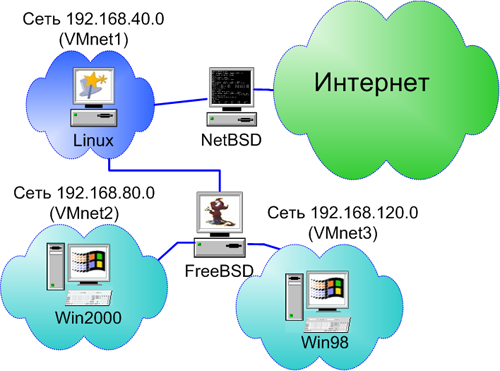
\includegraphics[scale=1]{res/network_general}
\caption{Рабочий макет стандартной схемы ККС.}
\end{figure}

Эмулируемая ККС имеет три сегмента (подсети)\footnote{Адрес подсети должен содержать маску! Далее будем полагать что речь идёт об /24 сетях.}:
\begin{itemize}
\item VMnet1 (адрес подсети – 192.168.40.0)
\item VMnet2 (адрес подсети – 192.168.80.0)
\item VMnet3 (адрес подсети – 192.168.120.0)
\end{itemize}

Сеть VMnet1 содержит основной многофункциональный сервер ККС (службы DHCP, DNS, Web, Proxy, почтовая, файловая и др.), использующий ОС Linux Mandrake. Сеть VMnet2 представлена хостом под управлением ОС Windows 2k (2000/XP/2003 Server) и имеет двойное назначение – она обеспечивает ККС дополнительным сервером и поддерживает Windows-клиент семейства 2k. Сеть VMnet3 объединяет рабочие станции c ограниченными аппаратными ресурсами, ориентированные на ОС Windows семейства 9x (95/98).

Взаимодействие сегментов ККС осуществляет маршрутизатор, обслуживаемый ОС семейства Unix (FreeBSD), а подключение ККС к внешней сети (Интернет или реальной сети учебной лаборатории) обеспечивает шлюз, реализуемый другой ОС семейства Unix (NetBSD).

Естественно, что каждый представитель подсетей (VMnet1, Vmnet2, VMnet3) имеет один сетевой адаптер, шлюз – два, а маршрутизатор – три сетевых адаптера.

Для определённости будем считать, что ККС использует смешанное (и статическое, и динамическое) распределение IP-адресов. 

Хост WIN98 (здесь и далее имя хоста формируется от названия гостевой ОС) имеет статический адрес 192.168.120.15, хост LINUX также имеет статический адрес – 192.168.40.32, а хост WIN2000 получает адрес 192.168.80.128 динамически с помощью виртуального сервера DHCP (встроенного по умолчанию в каждый сегмент сети, эмулируемой в среде VMware Workstation).

\begin{figure}[h!]
\centering
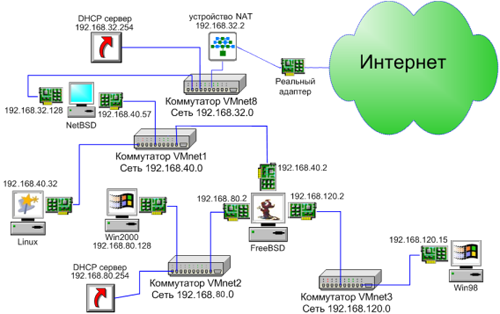
\includegraphics[scale=1]{res/network_general2}
\caption{Стандартная схема ККС.}
\end{figure}

Целесообразно выделить статические адреса для хостов FREEBSD (маршрутизатор) и NETBSD (шлюз). Для простоты адресам всех сетевых адаптеров маршрутизатора назначим одинаковые суффиксы – 192.168.40.2 (для связи с сетью VMnet1), 192.168.80.2 (для связи с сетью VMnet2), 192.168.120.2 (для связи с сетью VMnet3). Функциональное назначение шлюза (обеспечение взаимодействия ККС с внешними сетями) предполагает наличие какого-нибудь механизма сопряжения IP-адресов. Таким механизмом является служба NAT (преобразование сетевых адресов), подключённая к вспомогательной сети VMnet8, в которую (кроме устройства NAT) входит DHCP-сервер и шлюз. Адрес «внешнего» сетевого адаптера шлюза назначается динамически (DHCP-сервером сети VMnet8) – 192.168.32.128, а  адрес «внутреннего» сетевого адаптера шлюза (входящего в сеть VMnet1) статически – 192.168.40.57.

В результате всех подключений имеем схему ККС, представленную на рисунке 2.

%------------------------------------------------------------------------------
\newpage
\section{Эмуляция ККС в среде VirtualBox}

Эмуляция ККС считается завершенной, если выполнены следующие этапы:
\begin{itemize}
\item создание и настройка виртуальных сетей
\item создание и настройка виртуальных хостов
\end{itemize}

\subsection{Создание и настройка виртуальных сетей}

Построим вспомогательную сеть VMnet8 при помощи хост-машины, которая будет через NAT обеспечивать доступ NetBSD к ресурсам сети Интернет.

Для этого в меню File выбираем пункт Preferences, а в открывшемся окне переходим на вкладку Networks (рисунок 3).

\begin{figure}[h!]
\centering
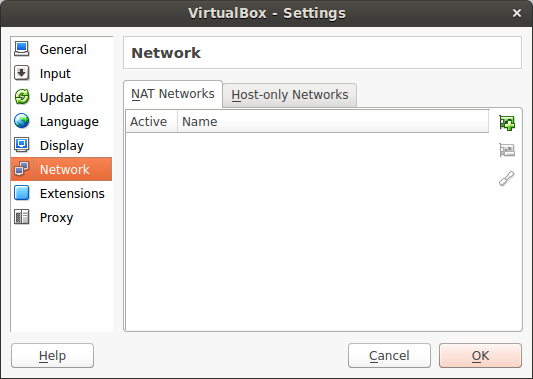
\includegraphics[scale=0.8]{res/virtualbox-networks}
\caption{Настройки сетевой системы VirtualBox.}
\end{figure}

При помощи кнопку со значком "+" добавим новую сетевую карту, которая будет обращена к виртуальной машине, а потом при помощи кнопки с отвёрткой сконфигурируем её так, как показано на рисунке 4.

\begin{figure}[h!]
\centering
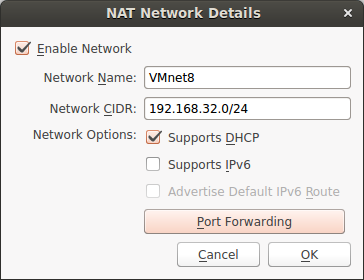
\includegraphics[scale=0.8]{res/virtualbox-nat}
\caption{Подготовка вспомогательной сети VMnet8.}
\end{figure}

Теперь создадим виртуальные машины (без установки и настройки) для прокладки виртуальных сетей. Для начала создадим NetBSD, используя стандартный шаблон, предлагаемый VirtualBox. Далее перейдём в сетевые настройки виртуальной машины и настроим первую сетевую карту для работы в режиме NAT через вспомогательную сеть VMnet8, как показано на рисунке 5.

\begin{figure}[h!]
\centering
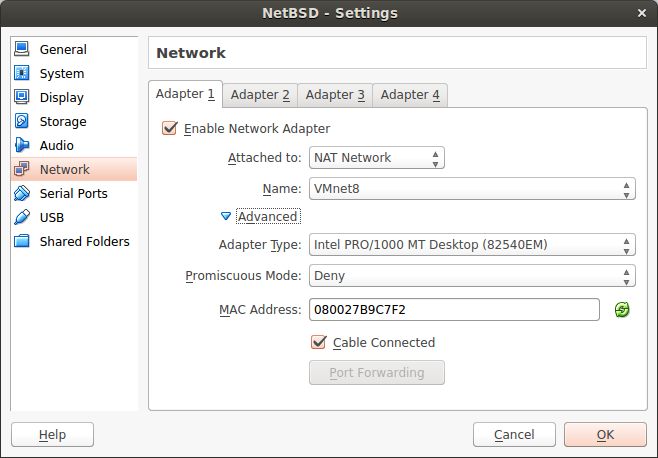
\includegraphics[scale=0.6]{res/netbsd-nat}
\caption{Настройка сетевого интерфейса NetBSD на работу с сетью VMnet8.}
\end{figure}

После этого можно перейти на вкладку с настройками для адаптера 2, включить его и обеспечить подключение к сети VMnet1 (рисунок 6).

\begin{figure}[h!]
\centering
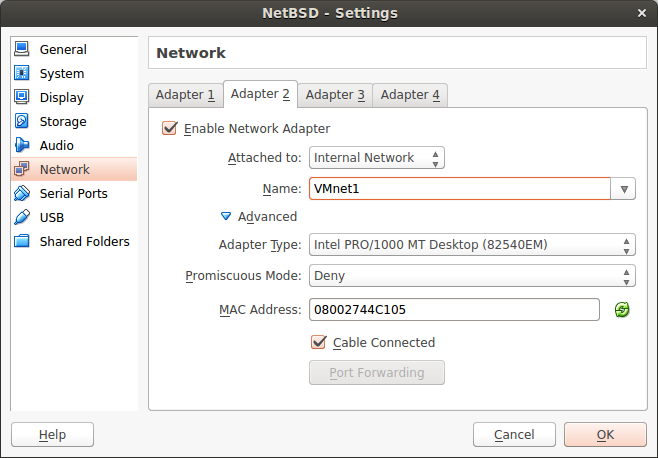
\includegraphics[scale=0.6]{res/netbsd-vmnet1}
\caption{Настройка второго сетевого интерфейса NetBSD на работу с сетью VMnet1.}
\end{figure}

После этого, пользуясь стандартными шаблонами и некоторыми оптимизациями, создадим ещё 4 виртуальные машины (Linux, FreeBSD, Win2000, Win98) и укажем в настройках их сетевых подключений ту сеть, к которой они должны быть подключены (аналогично подключению NetBSD к сети VMnet). При этом машина FreeBSD будет иметь три активированных сетевых адаптера (рисунок 7), и каждый из них будет взаимодействовать со своей виртуальной сетью.

Для организации DHCP в сети VMnet2, к сожалению, нет GUI-инструмента, но эта задача решается через командную строку:

\begin{Verbatim}[frame=single]
VBoxManage dhcpserver add --netname VMnet2 --ip 192.168.40.1 \
   --netmask 255.255.255.0 --lowerip 192.168.40.32 --enable
\end{Verbatim}

Удалить этот DHCP-сервер можно командой

\begin{Verbatim}[frame=single]
VBoxManage dhcpserver remove --netname VMnet2
\end{Verbatim}

\begin{figure}[h!]
\centering
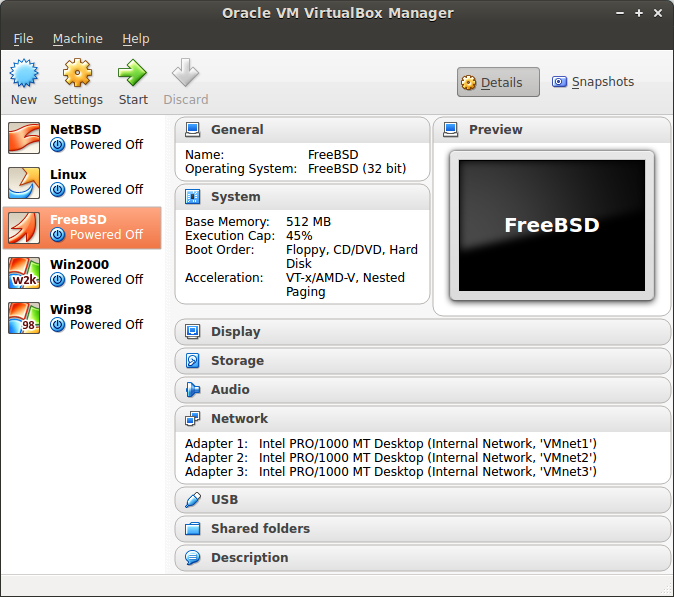
\includegraphics[scale=0.6]{res/freebsd-3net}
\caption{Три сетевые интерфейса, подключенные к разным сетям, на машине FreeBSD.}
\end{figure}

Как можно видеть выше, настройка выделенной виртуальной сети очень проста, для этого нужно только указать её имя. Эта простота компенсируется большей сложностью при создании и удалении DHCP-сервера для этой сети. Возможно в будущих версиях VirtualBox появятся более удобные инструменты для этого.

\newpage
\subsection{Создание и настройка виртуальных хостов}

Для эмуляции ККС требуется пять виртуальных хостов: Win98, Win200, Linux, FreeBSD, NetBSD.

Создание и настройка каждого виртуального хоста состоит из трёх этапов:
\begin{itemize}
\item создание виртуальной машины (этот шаг был проделан в процессе подготовки сети)
\item инсталляция гостевой операционной системы
\item конфигурация хоста в TCP/IP сети
\end{itemize}

Установка будет производиться с ISO-образов дистрибутивов. В целях экономии памяти, предпочтение будет отдаваться 32-х разрядным сборкам.

\subsubsection{Создание и настройка виртуального хоста NetBSD}

Установочный образ NetBSD 6.1.5 (NetBSD-6.1.5-i386.iso) скачиваем с официального сайта \url{http://www.netbsd.org/}.

В процессе установки, система задаст стандартные вопросы, типа предпочитаемого языка, параметров (геометрии) винчестера, желаемого вида установки. Задачей этого хоста является управление сетевым трафиком, следовательно нет необходимости в установке X11.

В процессе установки, система сама (при помощи DHCP) определила параметры интерфейса, который подключен к вспомогательной сети VMnet8 (см. рисунок 8)

\begin{figure}[h!]
\centering
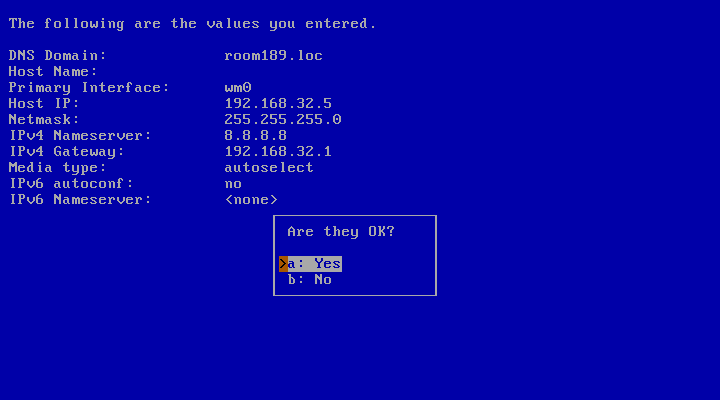
\includegraphics[scale=0.9]{res/netbsd-setup}
\caption{Автоматическое определение параметров сети в NetBSD.}
\end{figure}

После скачивания свежей версии портов (изначально wget отсутствует, так что свежие порты можно получить по ftp с \url{ftp.netbsd.org/pub/pkgsrc/stable/pkgsrc.tar.gz}) и установки удобного редактора, можно настроить сеть.

Для настройки второго сетевого интерфейса, в файл /etc/rc.conf нужно добавить строку
\begin{Verbatim}[frame=single]
ifconfig_wm1="inet 192.168.40.57 netmask 255.255.255.0"
\end{Verbatim}

Для включения ip-форвардинга, в файл /etc/sysctl.conf нужно добавить строку
\begin{Verbatim}[frame=single]
net.inet.ip.forwarding=1
\end{Verbatim}

Кроме того, потребовалось настроить некоторые демоны, такие как ipfilter (фаервол работает в режиме полного доступа, т.к. реальные задачи по ограничению доступа должны лежать на машине FreeBSD, выполняющей функции шлюза в локальную сеть) и ipnat (выполняет nat пакетов, предназначенных web-серверу и маскарадинг всех исходящих пакетов).

\begin{figure}[h!]
\centering
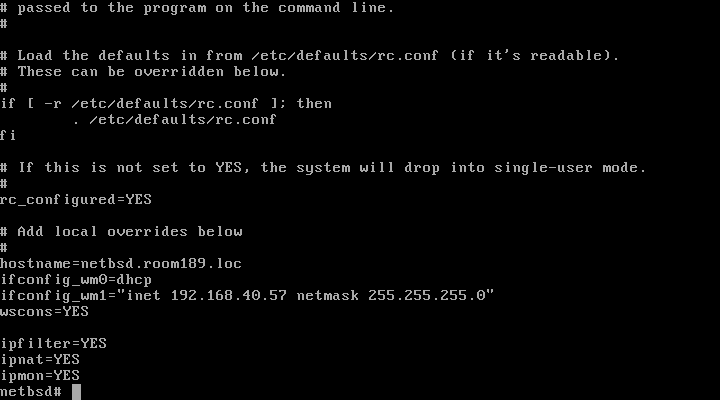
\includegraphics[scale=0.9]{res/netbsd-rcconf}
\caption{Файл инициализации rc.conf в NetBSD.}
\end{figure}

\subsubsection{Создание и настройка виртуального хоста Linux}

Последней версией Mandriva Linux на данный момент является версия 2014.1 (от 26 сентября 2014), установочный образ OpenMandriva.2014.0-kde4.i586.iso. После установки и исправления некоторых ошибок (директория /sbin не попала в переменную окружения \$PATH), выставим IP адрес и проверим работу системы.

Этот хост доступен снаружи по внешнему ip-адресу машины NetBSD, которая перенаправляет запросы, пришедшие на 80-й порт.

На рисунке 10 показана работа Mandriva Linux. В верхней части экрана присутствует вывод настроек сетевого подключения, в нижней - пинг до DNS-сервера Google.

\begin{figure}[h!]
\centering
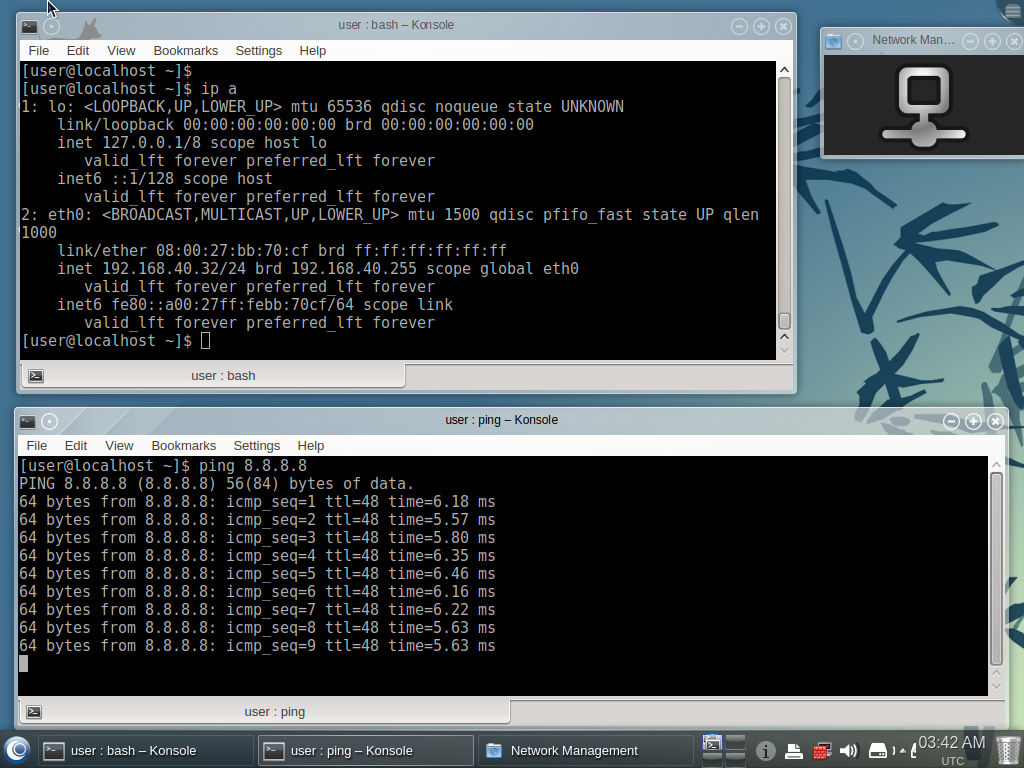
\includegraphics[scale=0.6]{res/linux-general}
\caption{Mandriva linux.}
\end{figure}

Стоит отметить, что в данном случае практически всё работает из коробки, пришлось настроить только IP-адрес. Очевидно, что Mandiva Linux с графической оболочкой KDE не лучший кандидат для корпоративного DHCP, DNS, Web, proxy, почтового и файлового сервера, не говоря уже о том, что эти роли нужно разносить по разным хостам.

\subsubsection{Создание и настройка виртуального хоста FreeBSD}

Как и NetBSD, FreeBSD весьма скромно потребляет ресурсы. В данном примере используется FreeBSD 10.1, установочный образ FreeBSD-10.1-RELEASE-i386-bootonly.iso, т.е. диск позволяет только загрузиться, вся система будет установлена путём скачивания с серверов FreeBSD.

Интересным моментом тут является то, что машина имеет три статически конфигурируемых интерфейса, а для обеспечения доступа из разных подсетей (к примеру, с машины Win98 к машине Win2000) не придётся явно прописывать маршрут, достаточно включить IP-форвардинг. На рисунке 11 представлен вывод файла /etc/rc.conf. Строка gateway\_enable обеспечивает включение форвардинга.

\begin{figure}[h!]
\centering
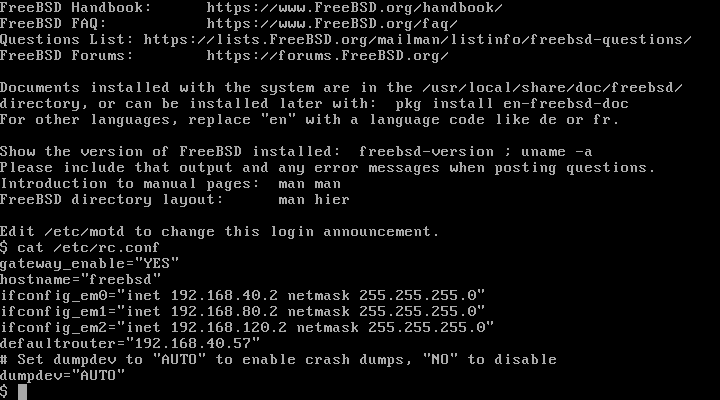
\includegraphics[scale=0.9]{res/freebsd-general}
\caption{FreeBSD.}
\end{figure}

\subsubsection{Создание и настройка виртуального хоста Win2000}

Машина с Windows 2000 получает свой IP динамически, его предоставляет DHCP-сервер, встроенный в VirtualBOox (его работа описывалась ранее).

После этого с Win200 можно отправить пинг на Linux, на все машины, для которых FreeBSD является шлюзом по умолчанию (т.е. это Linux и Win98), а также на саму машину FreeBSD. Отправка пинга на NetBSD (и далее в интернет) результата не даст, т.к. исходный хост (Win2000) находится в другом широковещательном домене. Чтобы NetBSD знала куда отвечать, на этой машине нужно добавить два маршрута (один для Win2000 и один для Win98):
\begin{Verbatim}[frame=single]
route add -net 192.168.80.0 -netmask 255.255.255.0 192.168.40.2
route add -net 192.168.120.0 -netmask 255.255.255.0 192.168.40.2
\end{Verbatim}

Кроме того, на NetBSD ещё нужно включить NAT для сети VMnet2 и VMnet3:
\begin{Verbatim}[frame=single]
echo "map wm0 192.168.80.0/24 -> 192.168.32.5/32" >> /etc/ipnat.conf
echo "map wm0 192.168.120.0/24 -> 192.168.32.5/32" >> /etc/ipnat.conf
\end{Verbatim}

В результате Win2000 может общаться с внешним миром. На рисунке 12 в верхней части отображены текущие сетевые настройки машины, в левой части пинг на DNS-сервер гугла (8.8.8.8; пакет идёт через трансляцию сетевых адресов на NetBSD), а в правой - пинг на win98 (пакет идёт через FreeBSD и для этого не потребовалось никаких настроек роутинга).

\begin{figure}[h!]
\centering
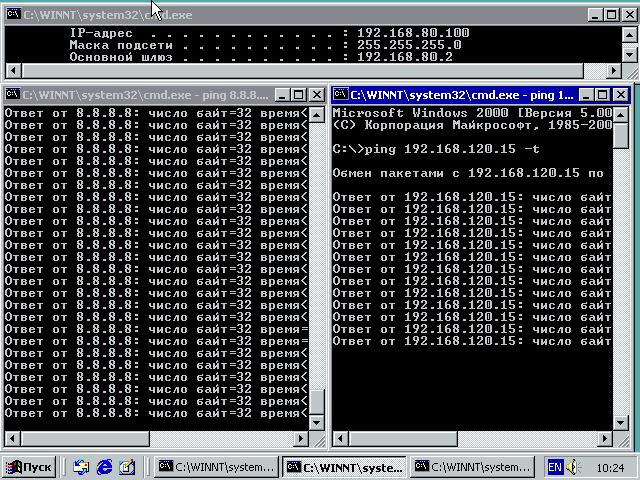
\includegraphics[scale=1]{res/win2000-general}
\caption{Win2000.}
\end{figure}

\subsubsection{Создание и настройка виртуального хоста Win98}

Ситуация с Win98 фактически аналогична ситуации с Win2000: эта машина также может отправлять пакеты всем хостам, для которых FreeBSD является шлюзом по умолчанию (и самой машине FreeBSD), а после дополнительных настроек маршрутизации и сетевой трансляции (рассмотренных выше) - отправлять пакеты в интернет.

Машина с Win98 получает свой адрес статически (рисунок 13).

\begin{figure}[h!]
\centering
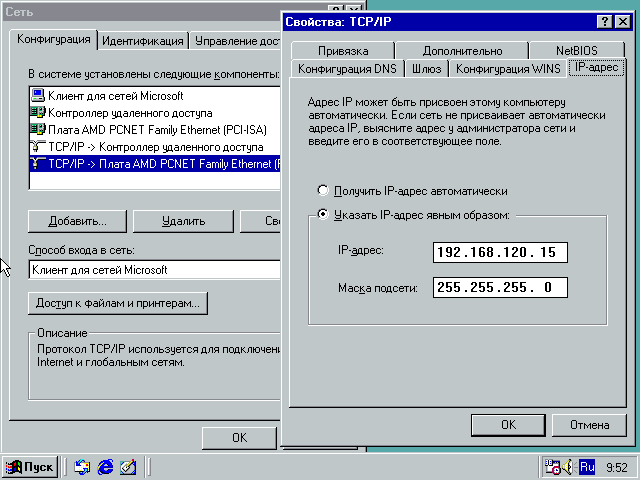
\includegraphics[scale=0.9]{res/win98-general}
\caption{Win98.}
\end{figure}

%------------------------------------------------------------------------------

\newpage
\section*{Заключение}
\addcontentsline{toc}{section}{Заключение}

В данной работе рассмотрен полунатуральный эмулятор корпоративной компьютерной сети (ККС). Он содержит три основных и один вспомогательный сегмент сети. Для построения этих сегментов используются механизмы, предоставляемые протоколом IP.

В работе приводятся результаты настройки различных систем (как современных так и морально устаревших):
\begin{itemize}
\item NetBSD (6.1.5);
\item FreeBSD (10.1);
\item Mandriva Linux (20014.0);
\item Windiws 2000;
\item Windows 98.
\end{itemize}

Приведены примеры использования некоторых сетевых технологий:
\begin{itemize}
\item Статическая адресация;
\item Динамическое выделение IP адреса;
\item Статическая и динамическая маршрутизация;
\item Трансляция сетевых адресов (NAT).
\end{itemize}

Подход с созданием полунатурального эмулятора корпоративной компьютерной сети вполне применим в реальной жизни, когда нужно заранее подготовить все конфиги (для быстрого и надёжного перехода или внедрения новой технологии) либо для расчёта отказоустойчивости, а также для проведения тестов на проникновение.

%------------------------------------------------------------------------------

\newpage
\section*{Список литературы}
\addcontentsline{toc}{section}{Список литературы}

\begin{enumerate}
\item Малышев И. А. - Методические указания по лабораторным работам по предмету «Администрирование компьютерных сетей».
\item Бешков А. VMware – виртуальный полигон для администратора и разработчика // Системный администратор, 2003, № 9.
\item Стахнов А. А. Сетевое администрирование Linux. – СПб: БХВ-Петербург, 2004.
\end{enumerate}

\end{document}